\section{Описание данных}
В качестве источника данных выбран датасет \href{https://www.kaggle.com/datasets/niteshyadav3103/concrete-compressive-strength}{Concrete Compressive Strength}. Данные содержат информацию о прочности бетона для определенного состава и возраста.

\textbf{Описание столбцов:}
\begin{enumerate}
	\item Cement -- содержание цемента ($\text{кг}/\text{м}^3$)
	\item Blast Furnace Slag -- содержание доменного шлака ($\text{кг}/\text{м}^3$)
	\item Fly Ash -- содержание летучей золы ($\text{кг}/\text{м}^3$)
	\item Water -- содержание воды ($\text{кг}/\text{м}^3$)
	\item Superplasticizer -- содержание пластификатора ($\text{кг}/\text{м}^3$)
	\item Coarse Aggregate -- содержание крупного заполнителя ($\text{кг}/\text{м}^3$)
	\item Fine Aggregate -- содержание мелкого заполнителя ($\text{кг}/\text{м}^3$)
	\item Age -- возраст бетона (дни)
	\item Concrete compressive strength -- прочность бетона на сжатие ($\text{МПа}$)
\end{enumerate}
\pagebreak

\section{Описание алгоритма}
\subsection*{Градиентный бустинг}
Градиентный бустинг --- ансамблевая модель машинного обучения, в котором базовые алгоритмы строятся последовательно, причем каждый следующий алгоритм старается уменьшить ошибку текущего ансамбля.

Рассмотрим обоснование градиентного бустинга для задачи регрессии с некоторой функцией потерь $\mathcal{L}(y_i, \hat{y_i})$. Пусть имеется обучающая выборка $X = \{x_i\},\ i = 1...N$ и целевая переменная $Y = \{y_i\},\ i = 1...N$. Для решения задачи будем строить композицию $a(x)$ из базовых алгоритмов $b(x)$.

$$a(x) = a_k(x) = b_1(x) + b_2(x) + \dots + b_k(x)$$

Композиция строится последовательно -- $a_k(x) = a_{k-1}(x) + b_k(x)$ -- добавляемый базовый алгоритм $b_k$ обучается так, чтобы улучшить предсказание текущего ансамбля.

$$b_k = \underset{b \in \mathcal{B}}{\mathrm{argmin}} \sum_{i=1}^N \mathcal{L}(y_i, a_{k-1}(x_i) + b(x_i))$$

Рассмотрим разложение функции потерь $\mathcal{L}$ в точке $(y_i, a_{k-1}(x) + b_k(x))$ в ряд Тейлора до первого члена в окрестности точки  $(y_i, a_{k-1}(x))$

$$\mathcal{L}(y_i, a_{k - 1}(x_i) + b(x_i)) \approx 
   \mathcal{L}(y_i, a_{k - 1}(x_i)) + b(x_i) \frac{\partial \mathcal{L}(y_i, z)}{\partial z} \bigg|_{z = a_{k - 1}(x_i)} 
   = \mathcal{L}(y_i, a_{k - 1}(x_i)) + b(x_i) g_i^{k - 1}$$

Таким образом, получаем следующую задачу оптимизации:

$$b_k \approx \underset{b\in \mathcal{B}}{\mathrm{argmin}} \sum_{i = 1}^N b(x_i) g_i^{k - 1}$$

Выражение, которое необходимо минимизировать, есть ни что иное, как скалярное произведение векторов $b(x)$ и $g^{k-1}$, поэтому его минимизируют значения $b(x_i)$ пропорциональные $-g_i^{k-1}$. То есть на каждой итерации базовый алгоритм $b_i(x)$ надо обучать так, чтобы он приближал значение антиградиента функции потерь для текущего ансамбля, что по сути является применением идеи градиентного спуска.

Аналогично с градиентным спуском, перемещение на значение антиградиента целиком может привести к проскакиванию минимума и потенциально вести к расхождению метода. Поэтому введем скорость обучения $\eta \in (0, 1]$, которая будет использовать для определения вклада базового алгоритма в композицию.

$$a_{k+1}(x) = a_{k}(x) + \eta b_{k+1}(x)$$

Потенциально, градиентный бустинг можно использовать с любым алгоритмом машинного обучения в качестве базового, но, например, для линейной модели результирующий ансамбль будет представлять из себя линейную комбинацию линейных моделей --- линейную модель. Поэтому традиционный базовый алгоритм для градиентного бустинга --- решающее дерево. 
\pagebreak

\section{Предобработка данных}
Данные не потребовали дополнительной предобработки. Они не содержат пропусков. Распределения признаков выглядят нормально, за исключением большого количества нулей у Furnace Slag, Fly Ash и Superplasticizer, которых однако слишком много, чтобы считать выбросами.

\begin{figure}[h]
\centering
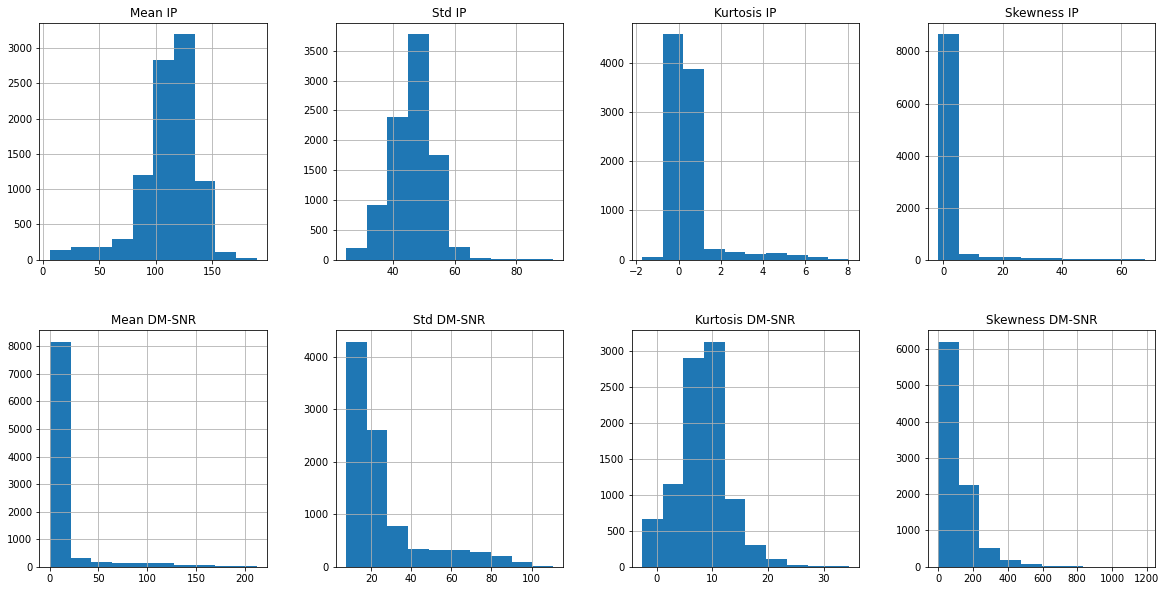
\includegraphics[width=.9\textwidth]{hist}
\caption{Гистограммы на основе значений признаков}
\end{figure}

Мультиколлинеарность также не наблюдается, поэтому в удалении каких-то признаков нет необходимости.

\begin{figure}[h]
\centering
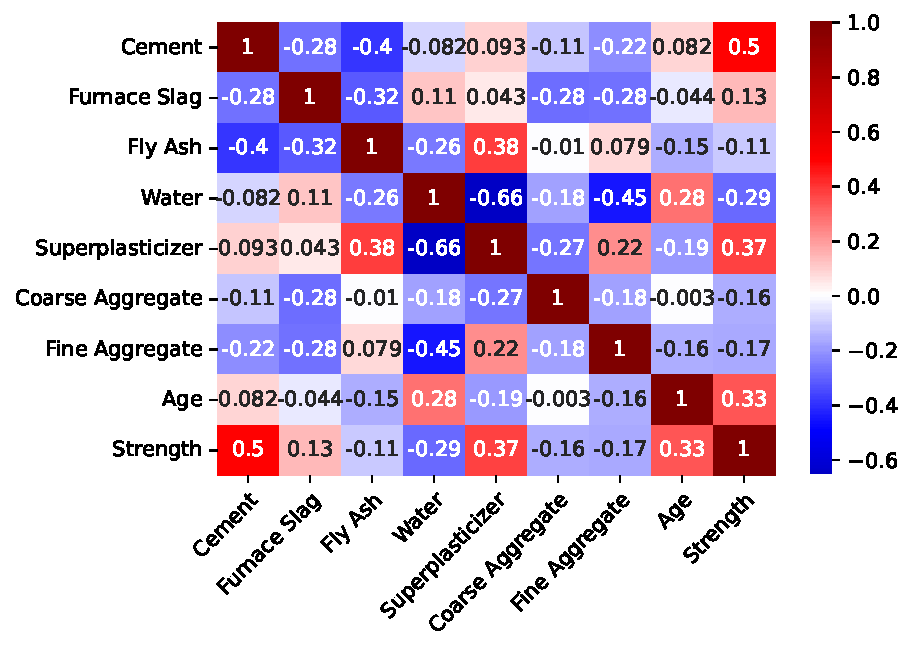
\includegraphics[scale=0.6]{corr}
\caption{Матрица корреляции признаков}
\end{figure}
\FloatBarrier

Единственная обработка данных, которая используется --- нормализация при помощи \texttt{sklearn.preprocessing.Normalizer} --- встроена в пайплайн каждой модели первым этапом.

\section{Реализация алгоритма}

Реализация решающего дерева не изменилась по сравнению с лабораторными работами. Настраиваемые гиперпараметры: глубина дерева, минимальный размер листа, способ вычисления ответа (среднее значение или медиана целевой переменной в листе) и критерий построения дерева. Реализованные критерии: среднеквадратичная ошибка, средняя абсолютная ошибка и среднее отклонение Пуассона.

\begin{lstlisting}[language=python, keepspaces=true]
class DecisionTree(BaseEstimator, RegressorMixin):
    class Node:
        def __init__(self):
            self.feature = -1
            self.value = None
            self.left = None
            self.right = None
    
    def __init__(self, min_leaf_size=5, max_depth=None, criterion='mse', answer='mean', features=None):
        self.min_leaf_size = min_leaf_size
        self.max_depth = max_depth
        self.criterion = criterion
        self.answer = answer
        self.features = features
    
    def fit(self, data, target):
        self.root = self.Node()
        self.process_node(data, target, self.root, np.arange(len(target)), 0)
        return self
    
    def crit(self, y_sum, y_sq_sum, y_med_sum, n):
        if self.criterion == 'mse':
            return y_sq_sum / n - y_sum ** 2 / n ** 2
        elif self.criterion == 'mae':
            return y_med_sum / n 
        elif self.criterion == 'poisson':
            return -y_sum / n * np.log(y_sum / n)
        
    def process_node(self, data, target, node, ids, depth):
        X = data[ids]
        Y = target[ids]
        n = len(X)
        y_sum = np.sum(Y)
        y_sq_sum = np.sum(Y ** 2)
        y_med = np.median(Y)
        y_med_sum = np.sum(np.abs(Y - y_med))
        
        if (self.max_depth is not None) and depth == self.max_depth or \
           (self.min_leaf_size is not None) and n <= self.min_leaf_size:
            if self.answer == 'mean':
                node.value = y_sum / n
            elif self.answer == 'median':
                node.value = y_med
            return
        
        h = self.crit(y_sum, y_sq_sum, y_med_sum, n)
        max_value = None
        max_f = None
        max_gain = -1
        best_left_ids = None
        best_right_ids = None
        for f in (self.features if self.features is not None else range(data.shape[1])):
            sort_ids = X[:, f].argsort()
            left = 1
            left_sum = Y[sort_ids[0]]
            left_sq_sum = Y[sort_ids[0]] ** 2
            left_med_sum = np.abs(Y[sort_ids[0]] - y_med)

            while left < n:
                while left < n and X[sort_ids[left-1]][f] == X[sort_ids[left-2]][f]:
                    left += 1
                    left_sum += Y[sort_ids[left-1]]
                    left_sq_sum += Y[sort_ids[left-1]] ** 2
                    left_med_sum += np.abs(Y[sort_ids[left-1]] - y_med)
                if left == n:
                    break
                    
                left_h = self.crit(left_sum, left_sq_sum, left_med_sum, left)
                right_h = self.crit(y_sum - left_sum, y_sq_sum - left_sq_sum, y_med_sum - left_med_sum, n - left)

                gain = h - (left * left_h + (n - left) * right_h) / n
                if gain > max_gain:
                    max_gain = gain
                    max_value = X[sort_ids[left-1]][f]
                    max_f = f
                    best_left_ids = sort_ids[:left]
                    best_right_ids = sort_ids[left:]

                left += 1
                left_sum += Y[sort_ids[left-1]]
                left_sq_sum += Y[sort_ids[left-1]] ** 2
                left_med_sum += np.abs(Y[sort_ids[left-1]] - y_med)
        
        if max_value is None:
            if self.answer == 'mean':
                node.value = y_sum / n
            elif self.answer == 'median':
                node.value = y_med
            return
        
        node.feature = max_f
        node.value = max_value
        node.left = self.Node()
        node.right = self.Node()
        
        self.process_node(X, Y, node.left, best_left_ids, depth+1)
        self.process_node(X, Y, node.right, best_right_ids, depth+1)
        
    def predict(self, data):
        res = np.ndarray(data.shape[0])
        for i, obj in enumerate(data):
            node = self.root
            while node.feature != -1:
                if obj[node.feature] > node.value:
                    node = node.right
                else:
                    node = node.left
            res[i] = node.value
        return res
\end{lstlisting}

Градиентный бустинг реализован с гиперпараметрами: количество деревьев, скорость обучения и функция потерь. Из функций потерь реализована только среднеквадратичная ошибка. Присутствует возможность обучать каждое дерево на подмножестве признаков и данных, но такой вариант показал себя плохо на данной задаче.
\begin{lstlisting}[language=python, keepspaces=true]
class GradientBoosting(BaseEstimator, RegressorMixin):
    def __init__(self, loss='mse', n_estimators=100, lr=0.1, max_features=1, subsample=1, **estimator_params):
        self.loss = loss
        self.n_estimators = n_estimators
        self.lr = lr
        self.max_features = max_features
        self.subsample = subsample
        self.estimator_params = estimator_params
        
    def negative_gradient(self, target, pred):
        if self.loss == 'mse':
            return target - pred
    
    def fit(self, data, target):
        features = np.arange(data.shape[1])
        if self.max_features == 'sqrt':
            max_features = int(np.floor(np.sqrt(len(features))))
        else:
            max_features = int(np.floor(len(features) * self.max_features))
        indexes = np.arange(len(data))
        samples = int(np.floor(self.subsample * len(data)))
        
        self.estimators = []
        pred = np.zeros(data.shape[0])
        for _ in range(self.n_estimators):
            if (self.max_features < 1):
                np.random.shuffle(features)
                
            self.estimators.append(DecisionTree(features=features[:max_features], **self.estimator_params))
            cur_target = self.negative_gradient(target, pred)
            if self.subsample < 1:
                idx = np.random.choice(indexes, (samples, ), replace=False)
                self.estimators[-1].fit(data[idx], cur_target[idx])
            else:
                self.estimators[-1].fit(data, cur_target)
            pred += self.lr * self.estimators[-1].predict(data)
        return self
    
    def predict(self, data):
        pred = np.zeros(data.shape[0])
        for tree in self.estimators:
            pred += self.lr * tree.predict(data)
        return pred
\end{lstlisting}

\pagebreak
